\section{Complicated Branching Structures}


   \subsection{Image Description}

     \begin{itemize}
         \item Image size: $1200 \times 1000$ pixels
         \item Surface area of shapes: $90000$ pixels
         \item Iterate the template $3, 4, 5, 6$ times to produce the targeted branching geometries labelled as $L_3, L_4, L_5, L_6$.
         \item Two groups of images labelled as $G_1, G_2$

           \begin{itemize}
             \item $G_1$: the target object $G_1 L_i$ ($i=3, 4, 5, 6$) is equidistant to the edges of an image.
             \item $G_2$: the template of $G_2 L_i$ ($i=3, 4, 5, 6$) is distinct from $G_1$ (thickness and aspect ratio). 
           \end{itemize}
           
     \end{itemize}



   \subsection{Output Analysis}


     \subsubsection{$S(n)$}



       \subsubsubsection{Estimated Survival Curves}

     
       \begin{figure}
        \centering
        
        \begin{subfigure}[b]{0.45\textwidth}
          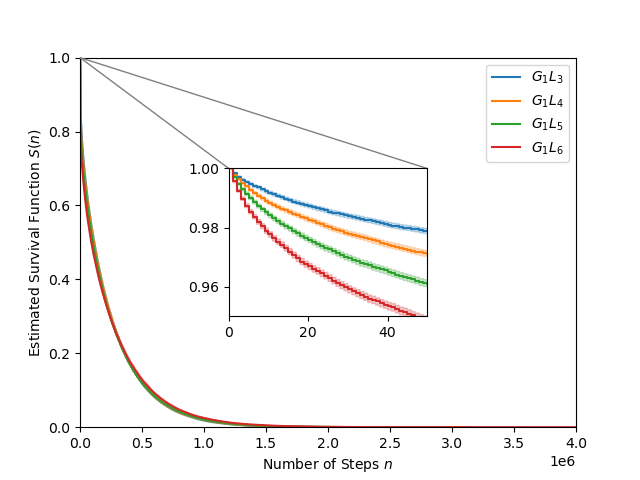
\includegraphics[width=\textwidth]{G_1_steps_sf.png}
          \caption{}
          \label{fig:sf_g1_branch_steps}
        \end{subfigure}
        \hfill
        \begin{subfigure}[b]{0.45\textwidth}
          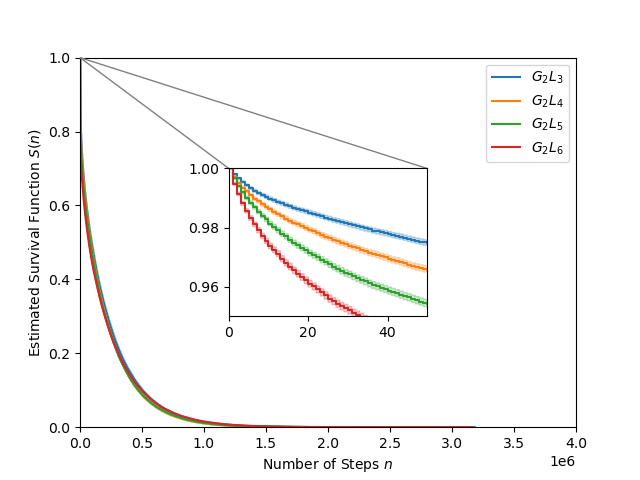
\includegraphics[width=\textwidth]{G_2_steps_sf.png}
          \caption{}
          \label{fig:sf_g2_branch_steps}
        \end{subfigure}

        \caption{}
        \label{fig:sf_branch_steps}

      \end{figure}



       \subsubsubsection{Non-Parametric Statistical Tests}

       
      \begin{table}
        \centering
        \begin{tabular}{llrrrr}
          \toprule
                       &             &         &  p &    &     \\
          \cmidrule{3-6}
                       &             & Logrank & TW & GB & FH  \\
          \midrule
          $G_1$ $L_3$  & $G_1$ $L_4$  &  0.4393 &  0.0285 &  0.0005 &  0.0005     \\
                       & $G_1$ $L_5$  & 0.0 & 0.0 & 0.0 & 0.0    \\
                       & $G_1$ $L_6$  & 0.0 & 0.0 & 0.0 & 0.0      \\
          $G_1$ $L_4$  & $G_1$ $L_5$  & 0.0007 & 0.0 & 0.0 & 0.0      \\
                       & $G_1$ $L_6$  & 0.0002 & 0.0 & 0.0 & 0.0       \\
          $G_1$ $L_5$   & $G_1$ $L_6$ & 0.7223 &  0.0 & 0.0 & 0.0      \\
          \bottomrule
        \end{tabular}
        \label{tab:g1_ingroup_tests_steps}
        \caption{}
      \end{table}


      \begin{table}
        \centering
        \begin{tabular}{llrrrr}
          \toprule
                       &             &         &  p &    &     \\
          \cmidrule{3-6}
                       &             & Logrank & TW & GB & FH  \\
          \midrule
          $G_2$ $L_3$  & $G_2$ $L_4$  &  0.0 &  0.0 &  0.0 &  0.0     \\
                       & $G_2$ $L_5$  & 0.0 & 0.0 & 0.0 & 0.0    \\
                       & $G_2$ $L_6$  & 0.0 & 0.0 & 0.0 & 0.0      \\
          $G_2$ $L_4$  & $G_2$ $L_5$  & 0.0016 & 0.0 & 0.0 & 0.0      \\
                       & $G_2$ $L_6$  & 0.0004 & 0.0 & 0.0 & 0.0       \\
          $G_2$ $L_5$   & $G_2$ $L_6$ & 0.7199 &  0.0 & 0.0 & 0.0      \\
          \bottomrule
        \end{tabular}
        \label{tab:g2_ingroup_tests_steps}
        \caption{}
      \end{table}



       \subsubsubsection{Mesurement of Dissimilarities for $S(n)$}
      

      \begin{figure}
        \centering
        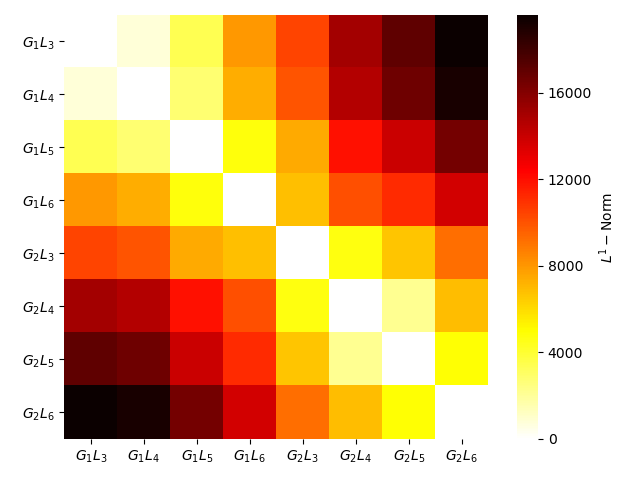
\includegraphics[width=\textwidth]{heatmap_ai_steps_l1.png}
        \caption{}
        \label{fig:heatmap_ai_steps_l1}
      \end{figure}

      
      \begin{figure}[h!]
        \centering
        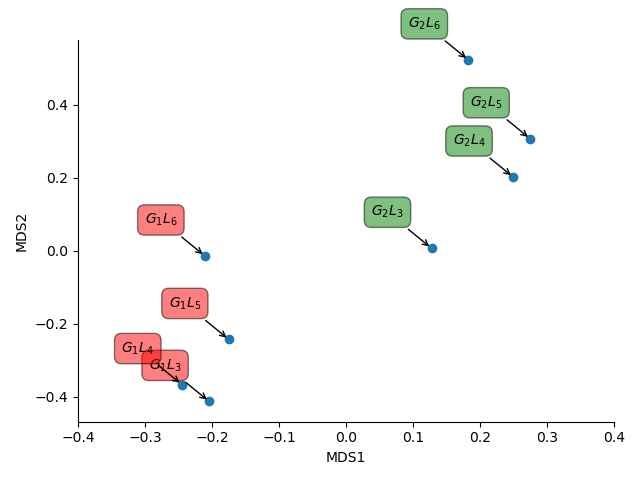
\includegraphics[width=\textwidth]{MDS_ai_steps_l1.png}
        \caption{}
        \label{fig:MDS_ai_steps_l1}
      \end{figure}
      


      
      \subsubsubsection{Visualize $S(n)$}

       \begin{figure}
         \centering
         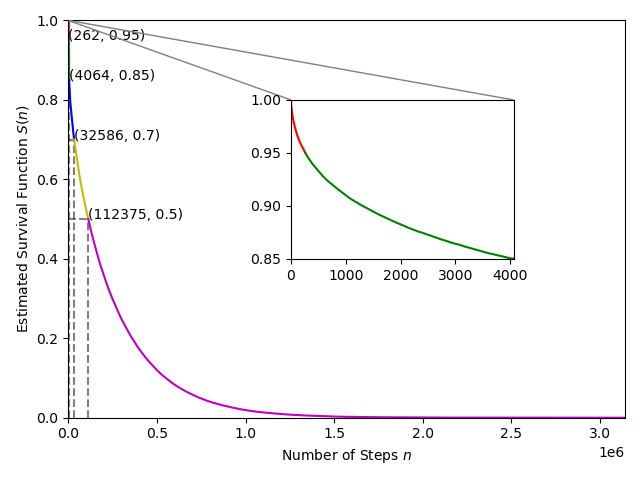
\includegraphics[width=\textwidth]{steps_seg_curve_G_1_L_3.png}
         \caption{}
         \label{fig:steps_seg_curve_G_1_L_3}
      \end{figure}



       \begin{figure}
         \centering
         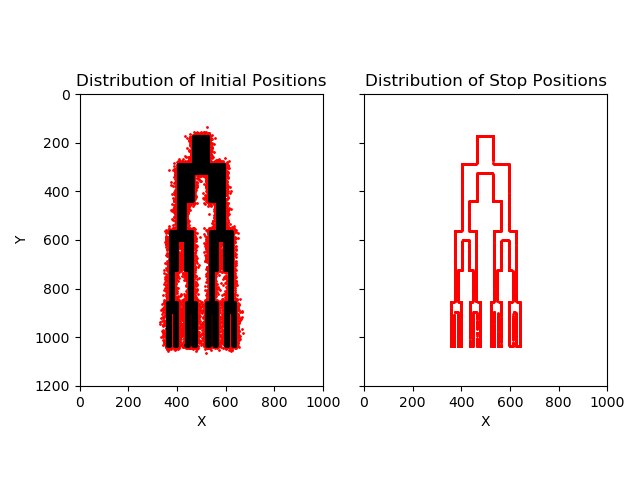
\includegraphics[width=\textwidth]{G_1_L_3_steps_red_initial_pos_distribution.png}
         \caption{}
         \label{fig:G_1_L_3_steps_red_initial_pos_distribution}
       \end{figure}



       \begin{figure}
         \centering
         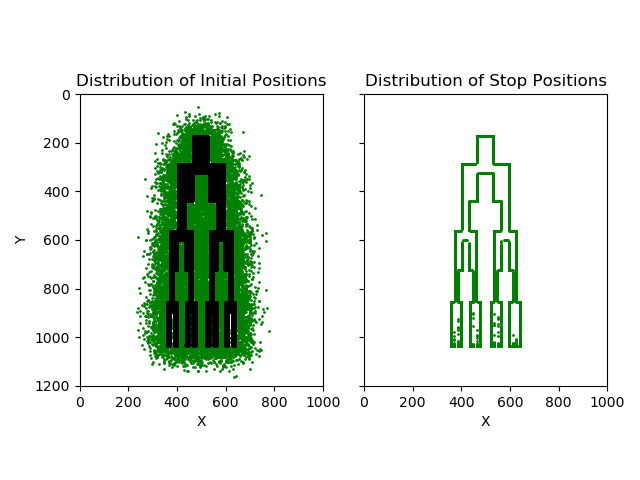
\includegraphics[width=\textwidth]{G_1_L_3_steps_green_initial_pos_distribution.png}
         \caption{}
         \label{fig:G_1_L_3_steps_green_initial_pos_distribution}
       \end{figure}


       \begin{figure}
         \centering
         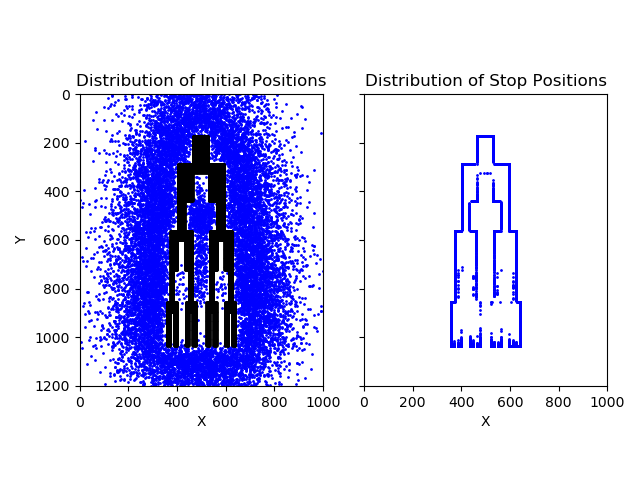
\includegraphics[width=\textwidth]{G_1_L_3_steps_blue_initial_pos_distribution.png}
         \caption{}
         \label{fig:G_1_L_3_steps_blue_initial_pos_distribution}
       \end{figure}
       

       \begin{figure}
         \centering
         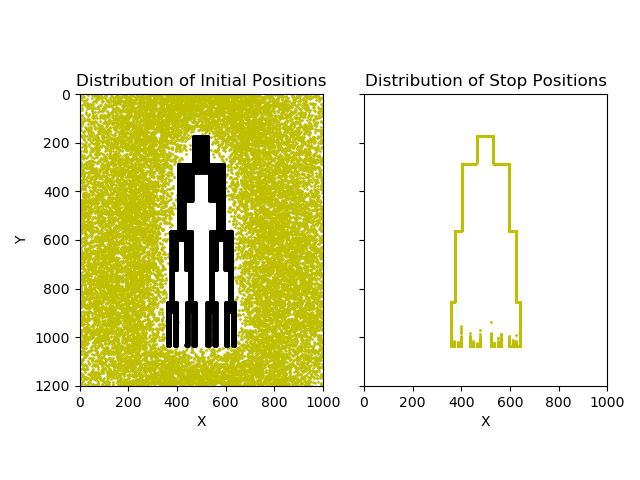
\includegraphics[width=\textwidth]{G_1_L_3_steps_y_initial_pos_distribution.png}
         \caption{}
         \label{fig:G_1_L_3_steps_y_initial_pos_distribution}
       \end{figure}


       \begin{figure}
         \centering
         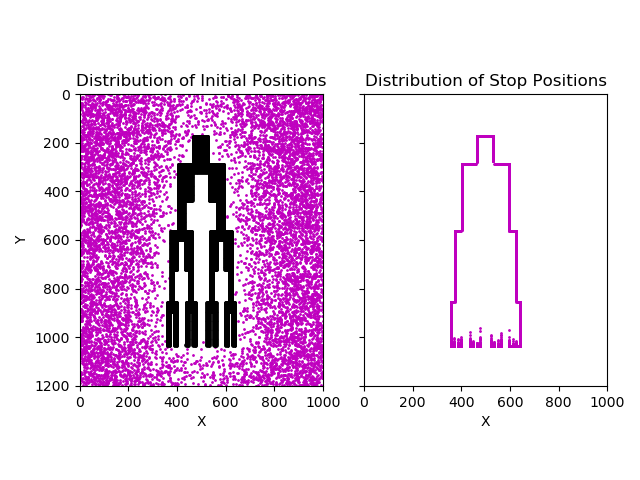
\includegraphics[width=\textwidth]{G_1_L_3_steps_m_initial_pos_distribution.png}
         \caption{}
         \label{fig:G_1_L_3_steps_m_initial_pos_distribution}
       \end{figure}


























      

      %____________________________________________________________



       \newpage

       
      \subsubsection{$S(d)$}



      \begin{figure}
        \centering
        
        \begin{subfigure}[b]{0.45\textwidth}
          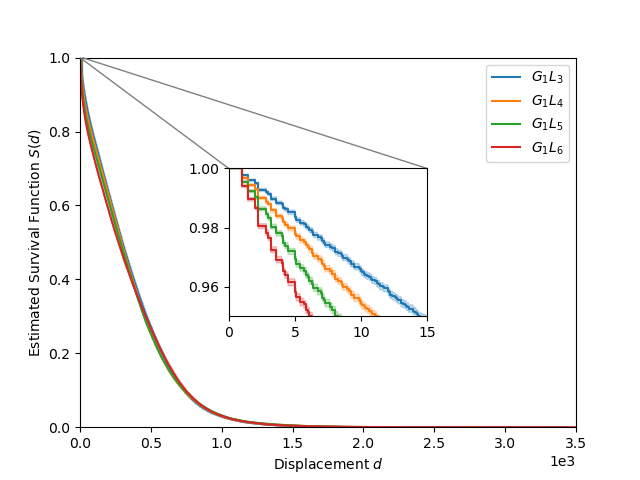
\includegraphics[width=\textwidth]{G_1_unwrap_disp_sf.png}
          \caption{}
          \label{fig:sf_g1_branch_disp}
        \end{subfigure}
        \hfill
        \begin{subfigure}[b]{0.45\textwidth}
          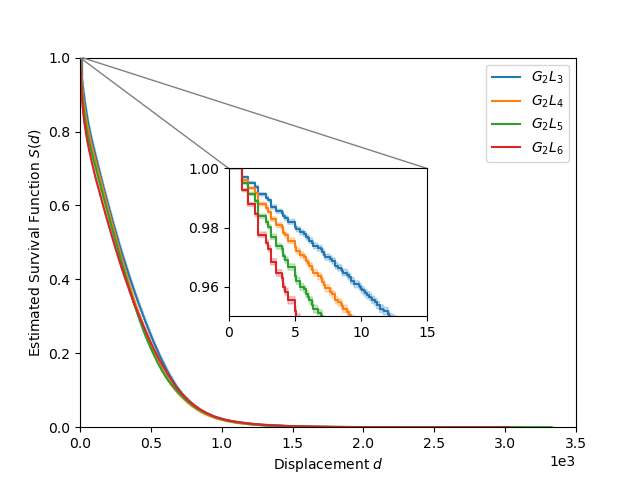
\includegraphics[width=\textwidth]{G_2_unwrap_disp_sf.png}
          \caption{}
          \label{fig:sf_g2_branch_disp}
        \end{subfigure}

        \caption{}
        \label{fig:sf_branch_disp}

      \end{figure}




      \begin{table}
        \centering
        \begin{tabular}{llrrrr}
          \toprule
                       &             &         &  p &    &     \\
          \cmidrule{3-6}
                       &             & Logrank & TW & GB & FH  \\
          \midrule
          $G_1$ $L_3$  & $G_1$ $L_4$  &  0.0 &  0.0 &  0.0 &  0.0     \\
                       & $G_1$ $L_5$  & 0.0 & 0.0 & 0.0 & 0.0    \\
                       & $G_1$ $L_6$  & 0.0 & 0.0 & 0.0 & 0.0      \\
          $G_1$ $L_4$  & $G_1$ $L_5$  & 0.0072 & 0.0 & 0.0 & 0.0      \\
                       & $G_1$ $L_6$  & 0.0003 & 0.0 & 0.0 & 0.0       \\
          $G_1$ $L_5$   & $G_1$ $L_6$ & 0.2883 &  0.0 & 0.0 & 0.0      \\
          \bottomrule
        \end{tabular}
        \label{tab:g1_ingroup_tests_disp}
        \caption{}
      \end{table}


      \begin{table}
        \centering
        \begin{tabular}{llrrrr}
          \toprule
                       &             &         &  p &    &     \\
          \cmidrule{3-6}
                       &             & Logrank & TW & GB & FH  \\
          \midrule
          $G_2$ $L_3$  & $G_2$ $L_4$  &  0.0 &  0.0 &  0.0 &  0.0     \\
                       & $G_2$ $L_5$  & 0.0 & 0.0 & 0.0 & 0.0    \\
                       & $G_2$ $L_6$  & 0.0 & 0.0 & 0.0 & 0.0      \\
          $G_2$ $L_4$  & $G_2$ $L_5$  & 0.0001 & 0.0 & 0.0 & 0.0      \\
                       & $G_2$ $L_6$  & 0.0015 & 0.0 & 0.0 & 0.0       \\
          $G_2$ $L_5$   & $G_2$ $L_6$ & 0.7019 &  0.0 & 0.0 & 0.0      \\
          \bottomrule
        \end{tabular}
        \label{tab:g2_ingroup_tests_disp}
        \caption{}
      \end{table}




      %______________________________________________________________
      

      \newpage
      

      \subsubsection{$S(R)$}
      
      \begin{figure}
        \centering
        
        \begin{subfigure}[b]{0.45\textwidth}
          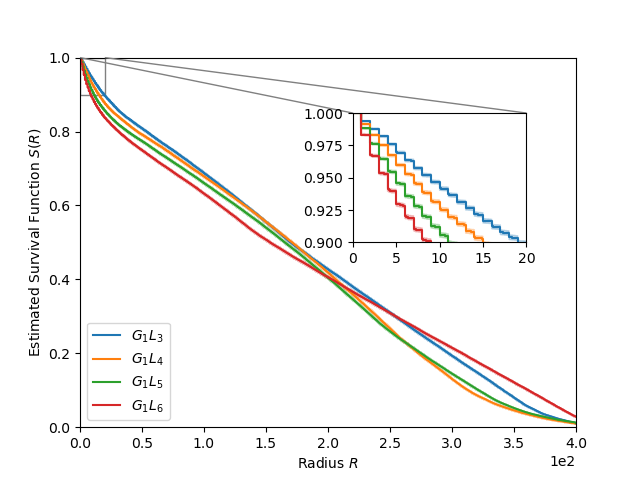
\includegraphics[width=\textwidth]{G_1_initial_radius_sf.png}
          \caption{}
          \label{fig:sf_g1_branch_radius}
        \end{subfigure}
        \hfill
        \begin{subfigure}[b]{0.45\textwidth}
          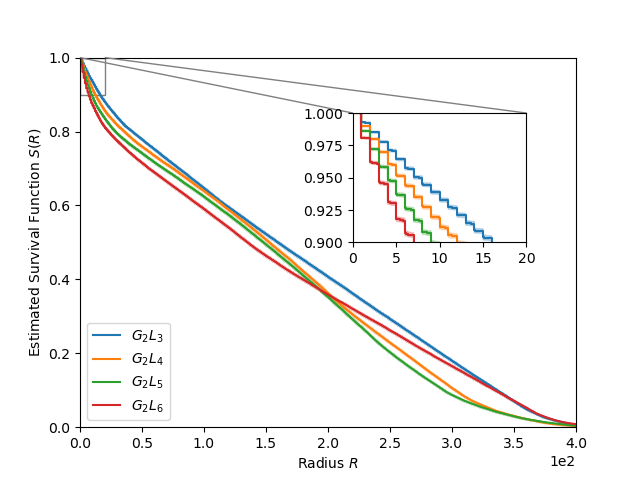
\includegraphics[width=\textwidth]{G_2_initial_radius_sf.png}
          \caption{}
          \label{fig:sf_g2_branch_radius}
        \end{subfigure}

        \caption{}
        \label{fig:sf_branch_radius}

      \end{figure}

      
      \begin{table}
        \centering
        \begin{tabular}{llrrrr}
          \toprule
                       &             &         &  p &    &     \\
          \cmidrule{3-6}
                       &             & Logrank & TW & GB & FH  \\
          \midrule
          $G_1$ $L_3$  & $G_1$ $L_4$  &  0.0 &  0.0 &  0.0 &  0.0     \\
                       & $G_1$ $L_5$  & 0.0 & 0.0 & 0.0 & 0.0    \\
                       & $G_1$ $L_6$  & 0.0 & 0.0 & 0.0 & 0.0      \\
          $G_1$ $L_4$  & $G_1$ $L_5$  & 0.1773 & 0.0 & 0.0 & 0.0      \\
                       & $G_1$ $L_6$  & 0.0 & 0.0 & 0.0 & 0.0       \\
          $G_1$ $L_5$   & $G_1$ $L_6$ & 0.0 &  0.0 & 0.0 & 0.0      \\
          \bottomrule
        \end{tabular}
        \label{tab:g1_ingroup_tests_radius}
        \caption{}
      \end{table}


      \begin{table}
        \centering
        \begin{tabular}{llrrrr}
          \toprule
                       &             &         &  p &    &     \\
          \cmidrule{3-6}
                       &             & Logrank & TW & GB & FH  \\
          \midrule
          $G_2$ $L_3$  & $G_2$ $L_4$  &  0.0 &  0.0 &  0.0 &  0.0     \\
                       & $G_2$ $L_5$  & 0.0 & 0.0 & 0.0 & 0.0    \\
                       & $G_2$ $L_6$  & 0.0 & 0.0 & 0.0 & 0.0      \\
          $G_2$ $L_4$  & $G_2$ $L_5$  & 0.0 & 0.0 & 0.0 & 0.0      \\
                       & $G_2$ $L_6$  & 0.0 & 0.0 & 0.0 & 0.0       \\
          $G_2$ $L_5$   & $G_2$ $L_6$ & 0.0 & 0.0 & 0.0253 & 0.0253      \\
          \bottomrule
        \end{tabular}
        \label{tab:g2_ingroup_tests_radius}
        \caption{}
      \end{table}


      


















    


      \newpage
      
    \subsection{Conclusion}

      \begin{itemize}
         \item In a short time, the survival function of rectangle decays faster than the circle, which conforms to the analytical results.
  
         \item The differences of estimated survival functions between circle and rectangle are statistically significant, which coincides with the real shape dissimilarities.

         \item Within a same group, when $t$ is small, the more branching the object is, the faster the survival function decays.

         \item Within a same group, the pairwise survival functions are statistically different.

         \item The corresponding target structures in $G_1$ and $G_3$ are invariant shapes under translation since their survival function are not statistically different. In other words, periodic boundary conditions of the image can eliminate the effect of the locations.

         \item LRWs can describe and classify the geometries, their spatial configurations, and the unoccupied area in the image.
    \end{itemize}




